\section{Results and Discussion}\label{sec:results}
Ik ben nog niet blij met dit gedeelte, maar ik heb het even zo gelaten. Wil graag andere plotjes maken voor de resultaten, heb tot nu toe alleen de mooie gifjes, maar die kunnen natuurlijk niet in de rapportage. Wil binnenkort alles opnieuw runnen en dan measures maken voor bijvoorbeeld percentage opgenomen waterstof, en dan een plotje maken van de hoeveelheid opgenomen waterstof in de tijd. Dat is denk ik een mooi resultaat. Doet Darcy ook. Maar voor nu snapshots van de plotjes:

\subsection*{Model 1}
For the first model of the perfectly stirred reactor, we can see the results in Figure~\ref{fig:model_one_result}. The density of the hydrogen gas decreases over time, while the density of the metal hydride increases over time. You see the rate of absorption decreasing over time, this is an effect of $\rho_g$ becoming smaller, and $\rho_s$ becoming larger. 
\begin{figure}
    \centering
    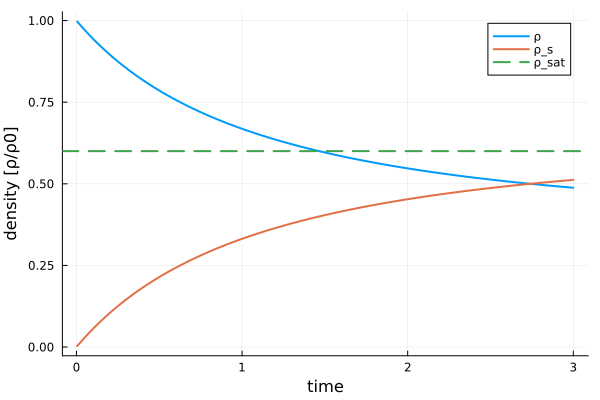
\includegraphics[width=0.6\textwidth]{figures/rho_plot.png}
    \caption{Plot of $\rho$ and $\rho_{sat}$ over time.}\label{fig:model_one_result}
\end{figure}

\subsection*{Model 2}
The results of this model after half a second are shown in Figure~\ref{fig:model_2_results}.

\begin{figure}[h]
    \centering
    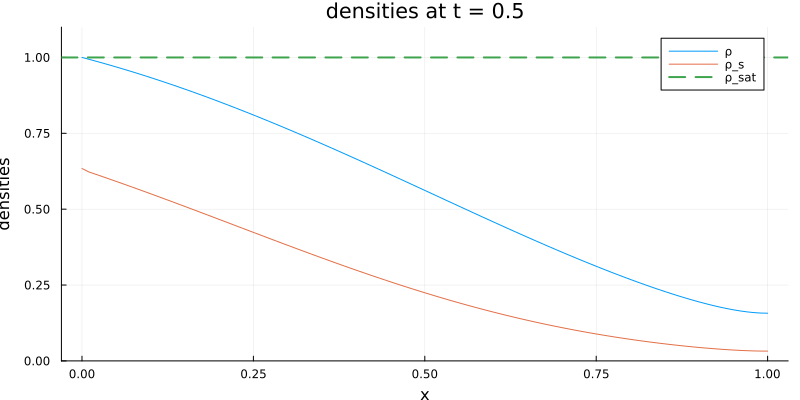
\includegraphics[width=0.8\textwidth]{figures/model_2_result.png}
    \caption{Results at $t=0.5$}\label{fig:model_2_results}
\end{figure}

\subsection*{Model 3}
The results of this model after one second are shown in Figure~\ref{fig:model_3_result}.

\begin{figure}
    \centering
    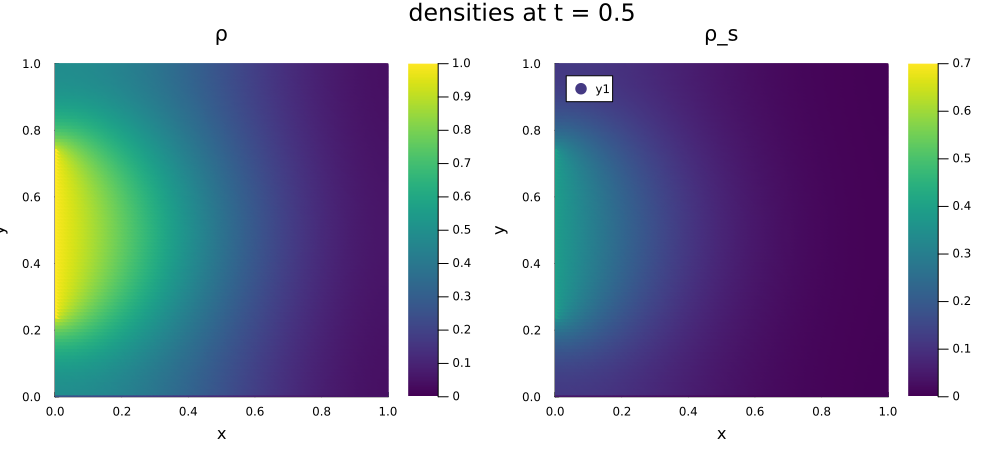
\includegraphics[width=.8\textwidth]{figures/model_3_result.png}
    \caption{Result of model 3 at time $t=1$}\label{fig:model_3_result}
\end{figure}

\subsection*{Model 4}
For the IMEX scheme we have visualized our results in Figure~\ref{fig:model_4_IMEX}, and for the Finite Difference scheme in Figure~\ref{fig:model_4_FD}. The results are similar, but the IMEX scheme is more stable and allows for larger time steps. The Finite Difference scheme requires smaller time steps to maintain stability, which can lead to longer computation times. Overall, the IMEX scheme provides a more efficient and robust solution for this model.

The result for applying total pressure is shown in Figure~\ref{fig:model_4_FD_ptot}. The total pressure is calculated using the formula above, and it shows how the pressure varies along the length of the battery at a specific time. The results indicate that the pressure is highest at the inlet and decreases towards the outlet, which is consistent with the expected behavior of the system.

\begin{figure}
    \centering 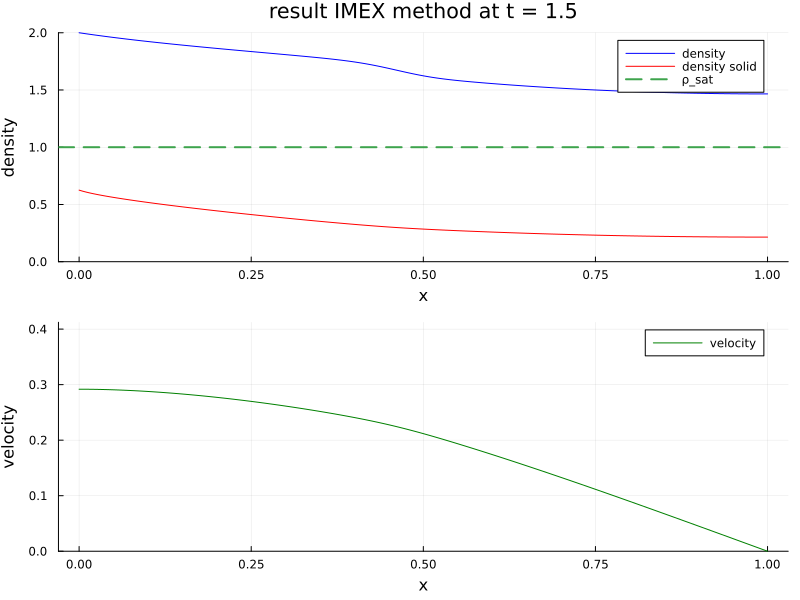
\includegraphics[width=.8\textwidth]{figures/model_4_result_IMEX.png}
    \caption{Results of the IMEX scheme at $t=1.5$.}\label{fig:model_4_IMEX}
\end{figure}

\begin{figure}
    \centering 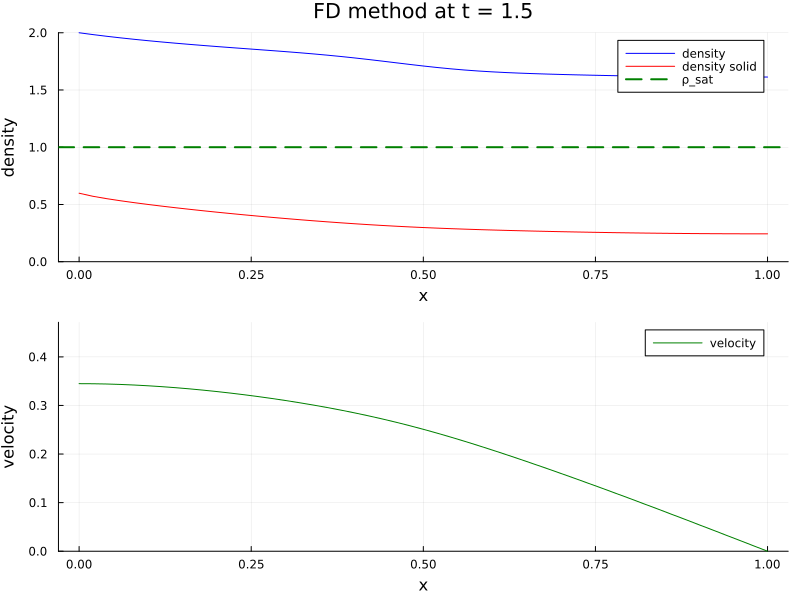
\includegraphics[width=.8\textwidth]{figures/model_4_FD.png}
    \caption{Results of the Finite Difference scheme at $t=1.5$.}\label{fig:model_4_FD}
\end{figure}

\begin{figure}
    \centering 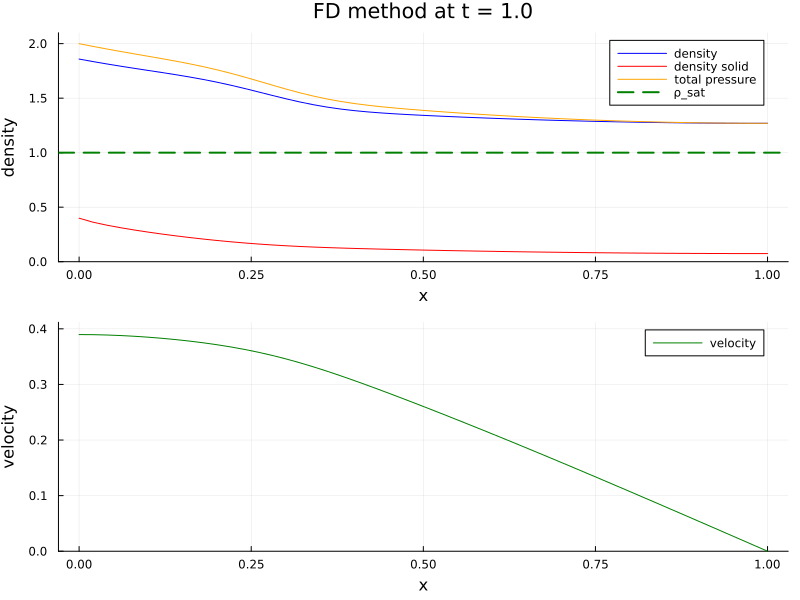
\includegraphics[width=.8\textwidth]{figures/model_4_FD_ptot.png}
    \caption{Results of the Finite Difference scheme with total pressure at $t=1.5$.}\label{fig:model_4_FD_ptot}
\end{figure}
